
%(BEGIN_QUESTION)
% Copyright 2006, Tony R. Kuphaldt, released under the Creative Commons Attribution License (v 1.0)
% This means you may do almost anything with this work of mine, so long as you give me proper credit

Bestem et par standardverdier for kondensator og motstand i denne op-amp-kretsen som vil gi et utgangssignal på 5 volt når inngangssignalet endrer seg med en jevn {\it rate} på 5 volt per sekund.

$$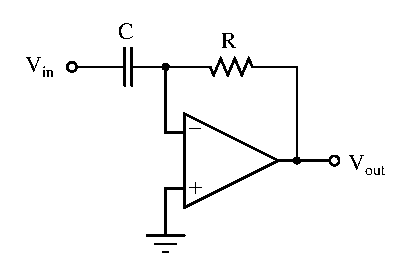
\includegraphics[width=15.5cm]{i01525x01.eps}$$

Med andre ord: dimensjoner denne deriveringskretsen slik at den får en {\it tidskonstant} på nøyaktig 1 sekund.

\underbar{file i01525}
%(END_QUESTION)





%(BEGIN_ANSWER)

Jeg lar deg finne et par komponentverdier på egen hånd! Det finnes ikke ett eneste ``riktig'' svar, siden et uendelig antall $RC$-kombinasjoner vil gi tidskonstanten $\tau_d$ = 1 sekund.

%(END_ANSWER)





%(BEGIN_NOTES)

$C$ = 1 $\mu$F og $R$ = 1 M$\Omega$ vil fungere.

%INDEX% Electronics review: differentiator circuit

%(END_NOTES)

